\begin{abstract}

We evaluate the explicit coefficient $C_0=1025$ for Wang\textquotesingle s support-size tester, conditional on the accompanying proof and with $L_0=1024$ unchanged. The frozen main design comprises 9,130,000 independent simulated Poisson-process paths and 39,720,000 paired method evaluations. Synthetic sizes range from $1$ to $10^{12}$ across five separation parameters and up to fifteen distribution scenarios. Ten published empirical populations cover trees, mites, birds, spiders, moths, snails, and fish. No errors are observed for $C_0=1025$ in the promised primary cells; worst simultaneous 95\% error upper bounds are 0.107\% on synthetic and 0.095\% on empirical populations. However, all practical sizes use the observed-count branch, a simple certified count baseline requires fewer samples, and only 2 of 236 ecological configurations have as many original records as the prescribed mean. Correlation stress tests expose violations of the iid requirement. Full-degree interval checks and public-API executions support implementation fidelity without substituting for a universal proof or a field validation.

\end{abstract}

\section{Question and claim boundaries}

We test the proposed constant reduction from $2^{26}$ to $1025$ in the supplied manuscript~\cite{wang}. For integer $n\ge1$, separation $0<\epsilon<1$, and $L=1+\log n$, the prescribed Poisson mean is $m=\lceil C_0n/(\epsilon L)\rceil$. The separation parameter $\epsilon$ is not the target error probability, which is $0.01$. Yes instances satisfy $S\le n$; No instances satisfy $\Delta_n(p)\ge\epsilon$. Gap instances satisfy neither promise and receive no classification-error label. We also check $\min\{\mathrm{eff}_\epsilon(p),n\}\le\widehat S\le S$ for every distribution, including Gap instances.

The coefficient reduction is an analytic refinement of the same construction, not a new asymptotic sample-complexity rate. Empirical evidence addresses finite tested distributions. It cannot establish uniform correctness over all distributions or integer minimality. In particular, $C_0=1024$ also succeeds on the tested practical grid; its theoretical obstruction lies near $n=e^{1023}\approx10^{444.28}$. The accompanying proof is included in the appendix for a precise statement of scope.

\section{Implementation and comparators}

The public reference interface now accepts an explicit sampling coefficient and records it in every output, while retaining the original coefficient as its default. Parameters, branch decisions, integer rounding and outputs are computed with Arb intervals and adaptive precision. The command \texttt{python paper\_reference.py demo --n 1000 --epsilon 0.1 --c0 1025} runs the new coefficient. All tested practical $n$ satisfy $L<1024$, so the literal algorithm is $D>n$ for rejection and $\widehat S=\min\{\max\{D,1\},n\}$. We do not force a polynomial branch at small $n$ or attribute tuned practical variants to this theorem.

Comparators are the original $C_0=2^{26}$ construction, $C_0=1024$ as a coefficient control, and a count baseline with the same 1\% target. For the latter, let $a=\log100$ and choose $m_{\rm count}=\lceil(n+a+\sqrt{a^2+2na})/\epsilon\rceil$. Discovery-time domination and a Poisson Chernoff bound certify its type-II error below 1\%; its type-I error is zero. This is a conservative analytic count baseline, not a data-tuned oracle. Constant sweeps below 1025 are sensitivity experiments without a claimed universal theorem.

\section{Experimental protocol and statistical analysis}

The primary grid uses $n\in\{1,2,10,10^2,10^3,10^4,10^6,10^9,10^{12}\}$ and $\epsilon\in\{0.001,0.01,0.05,0.1,0.25\}$. Scenarios include uniform and smaller-support nulls, dominant heads with extremely rare tails, piecewise power-law, lognormal, discrete Gaussian-shaped and geometric-shaped nulls, near-boundary uniform alternatives, diffuse and ultradiffuse tails, multiscale alternatives, clear alternatives, and two Gap controls. Blocked shapes are explicitly constructed discrete distributions, not claimed exact continuous Gaussian or lognormal laws. Invalid null variants at $n=1$ are omitted prospectively. Promise labels and effective-support integers are checked with rational arithmetic; empirical-data labels are additionally checked from integer counts.

Each primary distribution/parameter cell has four independent blocks of 2,500 trials. Methods share nested Poisson-process occupancies within a trial for paired comparisons. For a group of $g$ equal-probability categories, unseen categories are discovered over an increment $\Delta m$ by binomial thinning with probability $1-e^{-p\Delta m}$. This is the exact joint occupancy law in real arithmetic; numerical random generation uses binary64. It does not materialize the nominal sample stream or recover its realized length $M$. We save every method\textquotesingle s observed count, not just averages. The coefficient sweep uses 4,000 trials per cell and fourteen coefficients from 0.25 to 1025.

For $k$ failures in $T$ trials, we report the one-sided Clopper--Pearson upper bound $\operatorname{Beta}^{-1}(1-\alpha;k+1,T-k)$, with value one when $k=T$. Bonferroni adjustment sets $\alpha=0.05/K$ across all promised method cells within each suite. Lower-bound failures use a separate family over all cells, including Gap controls. These are suite-specific simultaneous statements, not a single global 95\% statement across every analysis. No trial count or parameter was changed in response to observed errors. A saved protocol amendment fixes duplicate output-log keys only; it does not change completed simulations. Supplemental API, runtime and group checks were separately recorded after primary summary inspection.

\section{Natural abundance data and validation targets}

We use abundance counts rather than biomass, percentage cover, or incidence frequencies. BCI trees and soil mites come from vegan~\cite{vegan}; birds and two spider treatments from iNEXT~\cite{inext}; moths and land snails from sads~\cite{sads}; seine-caught fish are stratified by year in InchLake1~\cite{fish}. Source commits, SHA256 digests, licensing notes and cleaning rules are saved in \texttt{data\_sources.json}. BCI refers to the 1982 large-tree subset, not a modern full-forest inventory. Historical abundance vectors have no recoverable event order. No species are invented to enlarge a real dataset.

\begin{table}[tbp]\centering\small\begin{tabular}{lrrr}\toprule Empirical population & Records & Species & Natural groups\\\midrule

Soil mites & 9,800 & 35 & 70\\

Birds (North) & 202 & 27 & --\\

Birds (South) & 307 & 38 & --\\

Spiders (Girdled) & 168 & 26 & --\\

Spiders (Logged) & 252 & 37 & --\\

Moths & 15,609 & 240 & --\\

Land snails & 1,689 & 21 & --\\

Forest trees & 21,457 & 225 & 50\\

Fish (2007 seine) & 1,180 & 8 & 15\\

Fish (2008 seine) & 330 & 4 & 15\\

\bottomrule\end{tabular}\caption{Published finite populations. Groups are spatial plots, soil cores or capture events; separate bird sites and spider treatments are not pooled.}\end{table}

The confirmatory numerical target is each cleaned empirical distribution $\widehat p_i=c_i/\sum_j c_j$. Independent Poisson resampling provides known finite truth, but cannot discover species absent from the source file. For each $\epsilon$, thresholds are the unique positive values among $\lfloor S/2\rfloor$, $\mathrm{eff}_\epsilon-1$, $\mathrm{eff}_\epsilon$, $S$, and $\lceil1.5S\rceil$. Truth is used to construct a benchmark and score results; the decision interface receives only the observed fingerprint and predeclared $n,\epsilon,m$. This is not a deployment procedure for choosing $n$ from an unknown ecosystem.

\begin{figure}[tbp]\centering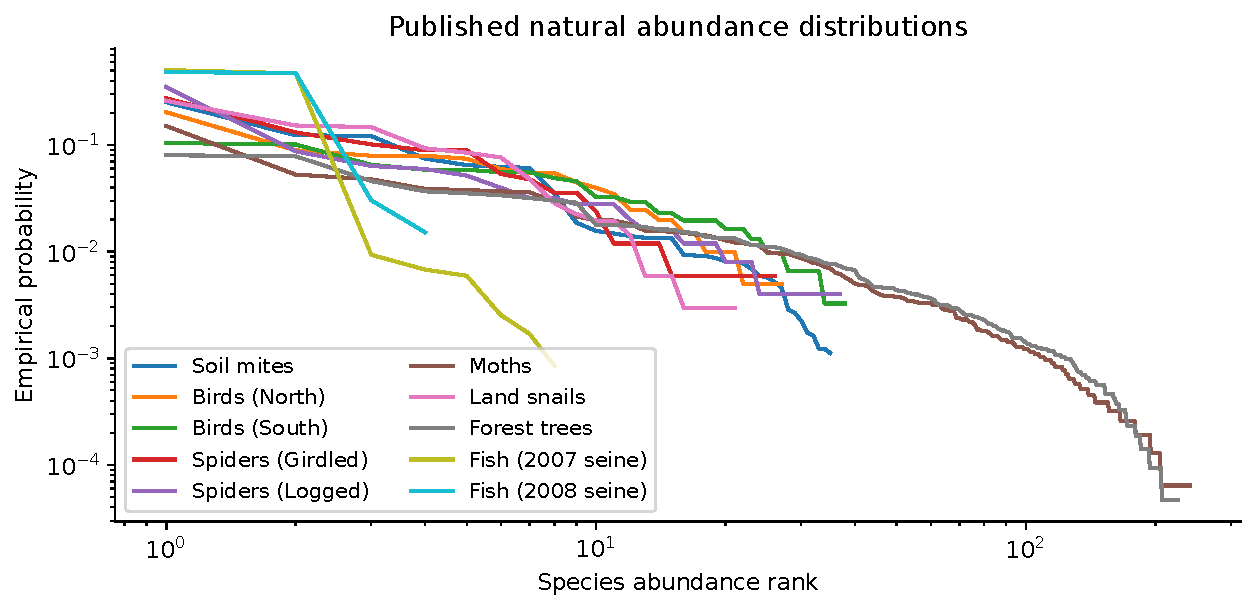
\includegraphics[width=.96\linewidth]{figures/natural_shapes.pdf}\caption{Rank-abundance distributions for ten published empirical populations spanning seven biological groups. These are observed finite populations, not complete ecosystem inventories.}\end{figure}

\section{Risk and acquisition-budget results}

\begin{table}[tbp]\centering\small\begin{tabular}{llrrr}\toprule Suite & Method & Errors / trials & Worst error & Simultaneous upper\\\midrule

Synthetic & C = 1024 & 0/5,550,000 & 0.000\% & 0.107\%\\

Synthetic & C = 1025 & 0/5,550,000 & 0.000\% & 0.107\%\\

Synthetic & Original C = 2\textasciicircum{}26 & 0/5,550,000 & 0.000\% & 0.107\%\\

Synthetic & 99\% count baseline & 203/5,550,000 & 0.130\% & 0.347\%\\

Natural & C = 1024 & 0/1,760,000 & 0.000\% & 0.095\%\\

Natural & C = 1025 & 0/1,760,000 & 0.000\% & 0.095\%\\

Natural & Original C = 2\textasciicircum{}26 & 0/1,760,000 & 0.000\% & 0.095\%\\

Natural & 99\% count baseline & 0/1,760,000 & 0.000\% & 0.095\%\\

\bottomrule\end{tabular}\caption{Errors on promised instances. ``Worst error'' is the largest cellwise observed rate, not a pooled rate. Confidence families include all methods in the respective suite.}\end{table}

The main experiment comprises 645 synthetic cells and 236 empirical cells, each evaluated by four methods. The C1025 joint lower-bound failure upper limits are 0.108\% and 0.098\%, respectively, below the theorem\textquotesingle s 2\% joint target. The count baseline also meets the 1\% error target on the tested grid. Thus the experiments support implementation correctness and conservative guarantees, not practical sample-efficiency dominance.

Across the synthetic grid, the C1025 budget is 35.8--135.2 times the count-baseline budget. Reducing the original coefficient changes its prescribed mean by approximately 65,472 times; this does not imply an equal wall-clock speedup or equal savings relative to a stronger finite-scale baseline. The coefficient sweep finds much smaller sufficient tested constants on its restricted scenarios. Such selected grid values are not universal optima.

\begin{figure}[tbp]\centering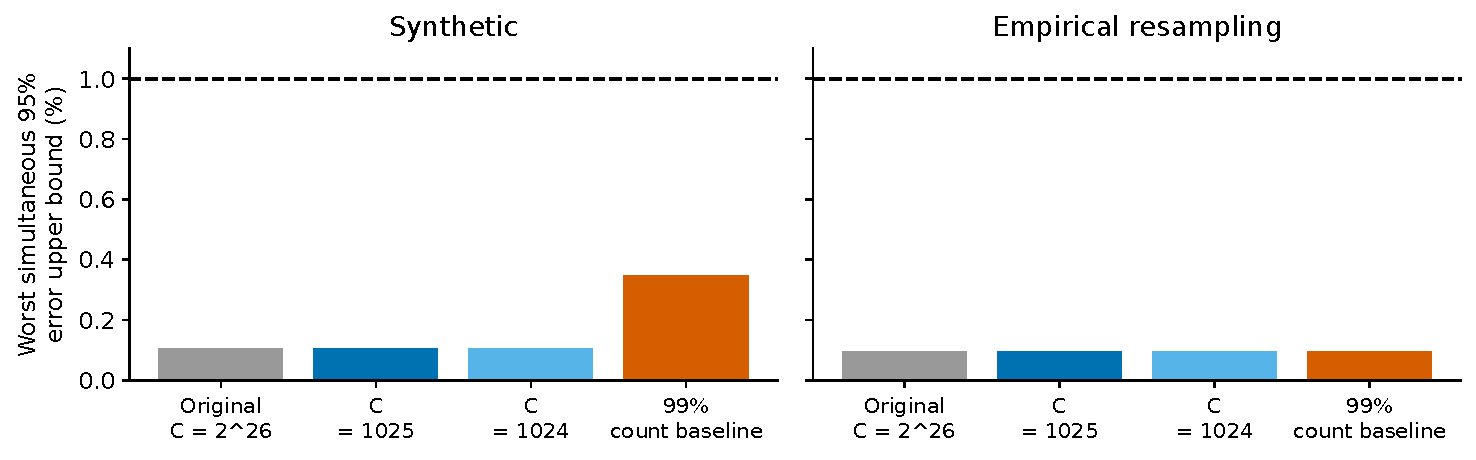
\includegraphics[width=.96\linewidth]{figures/risk.pdf}\caption{Worst cellwise error upper confidence bounds, Bonferroni-adjusted within each suite over all promised method cells. Zero observed errors are not zero risk.}\end{figure}

\begin{figure}[tbp]\centering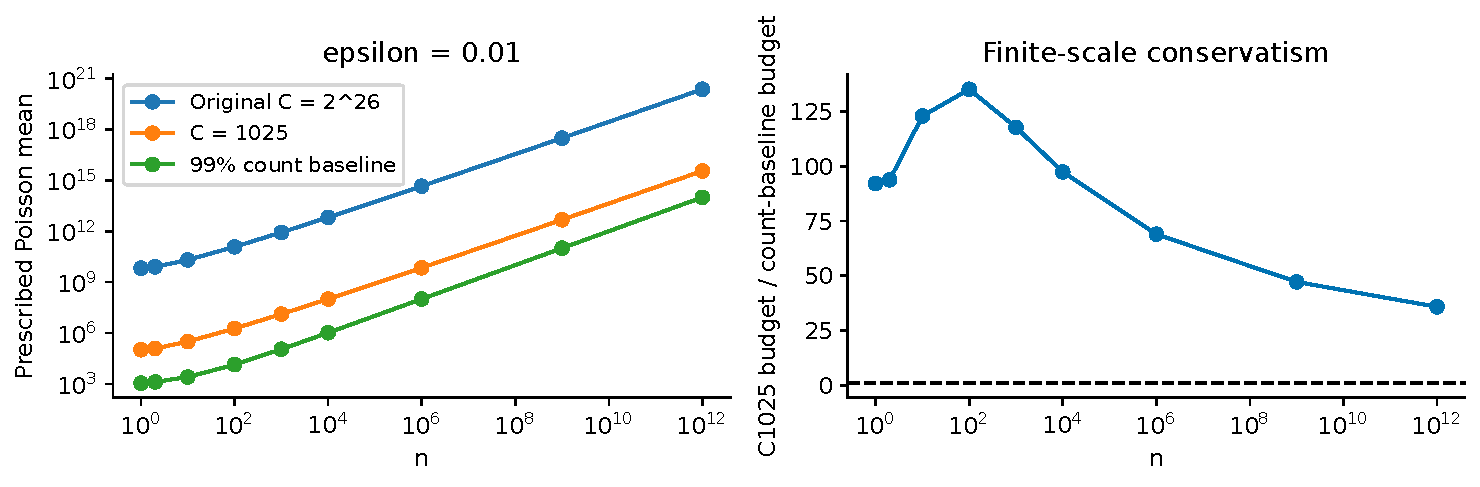
\includegraphics[width=.96\linewidth]{figures/budgets.pdf}\caption{Prescribed acquisition budgets, not simulator run times. The original coefficient decreases by about 65,472x, but a 99\% Chernoff count baseline remains cheaper over all tested sizes.}\end{figure}

\begin{figure}[tbp]\centering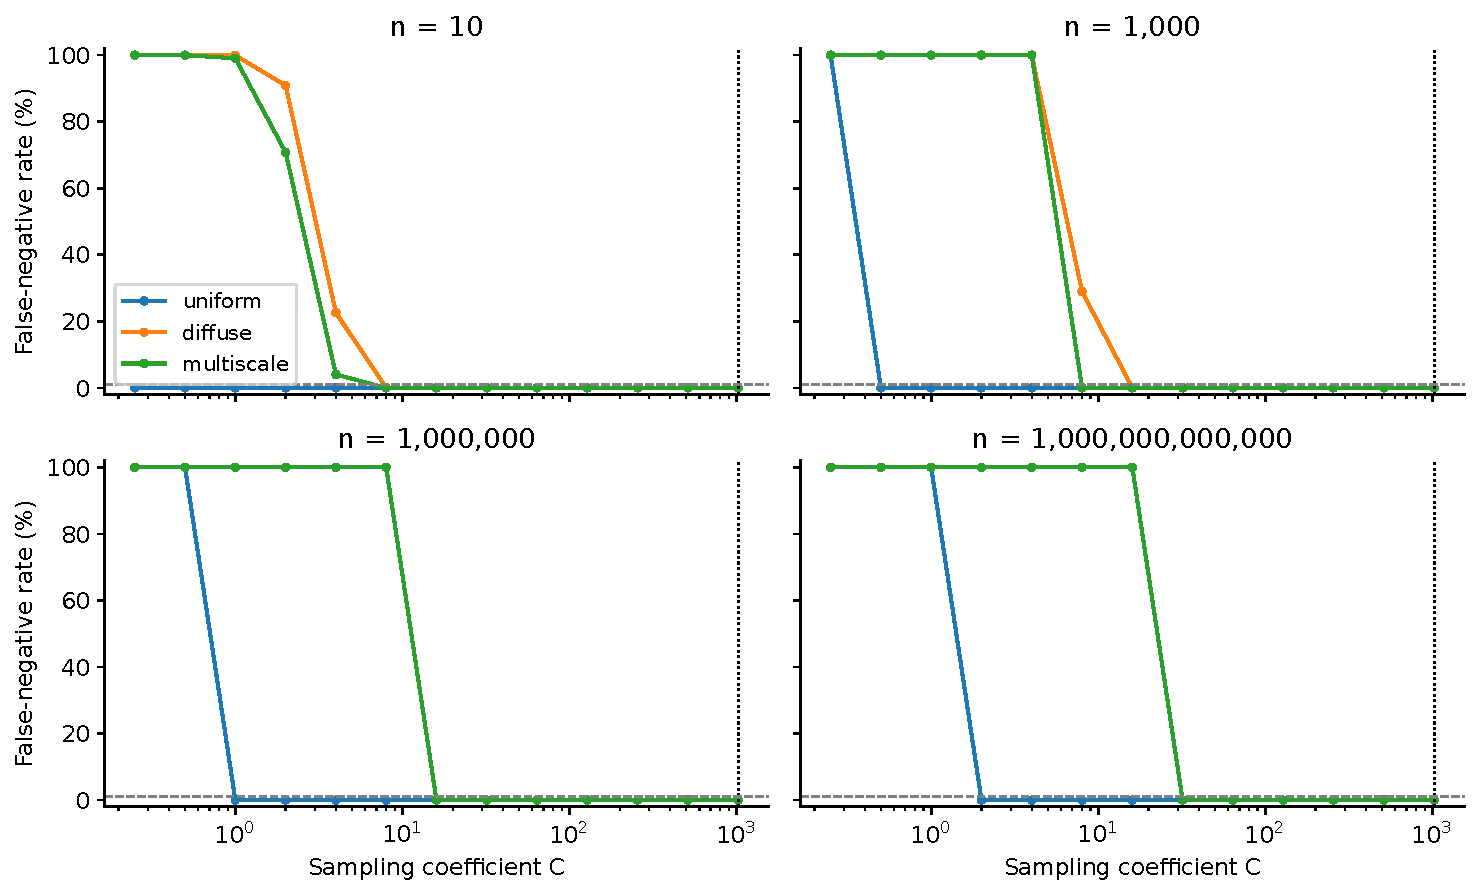
\includegraphics[width=.96\linewidth]{figures/constant_sweep.pdf}\caption{Coefficient sensitivity for three alternatives at epsilon=0.01. Each point has 4,000 trials; the CSV includes simultaneous confidence bounds. Dashed horizontal line: 1\% target. Vertical dotted line: C=1025.}\end{figure}

\section{What can the original ecological records validate?}

Only 2/236 ecological configurations have $N\ge m_{1025}$. We also report $\Pr\{\operatorname{Poi}(m)>N\}$, because $N\ge m$ alone does not guarantee a feasible Poisson draw. The only mean-feasible configurations are from the mite dataset. We run 200 finite-file Poisson subsampling attempts for each and retain every overflow rather than redrawing. These without-replacement file analyses are descriptive: the underlying spatial core collection has not been established to be an iid sample from the desired external population. For insufficient files, resampling with replacement does not create additional independent ecological evidence.

In the mite configurations, $(n,\epsilon,m,N)=(6,0.25,8812,9800)$ and $(7,0.25,9743,9800)$. The first has no overflows in 200 attempts; the second has 52 in 200, consistent with its nominal overflow probability of about 0.280. Both thresholds already lie below the 35 observed species, so these runs do not establish previously unknown ecological richness or certified acceptance.

Observing more than $n$ valid species directly refutes $S\le n$ without an iid assumption. Conversely, seeing at most $n$ species in an inadequate or biased survey does not certify acceptance. In particular, neither a high empirical resampling success rate nor an algorithmic Yes proves a complete species inventory. Sampling effort, detection bias, spatial clustering and the chosen biological sampling unit must be specified for a field application.

\begin{figure}[tbp]\centering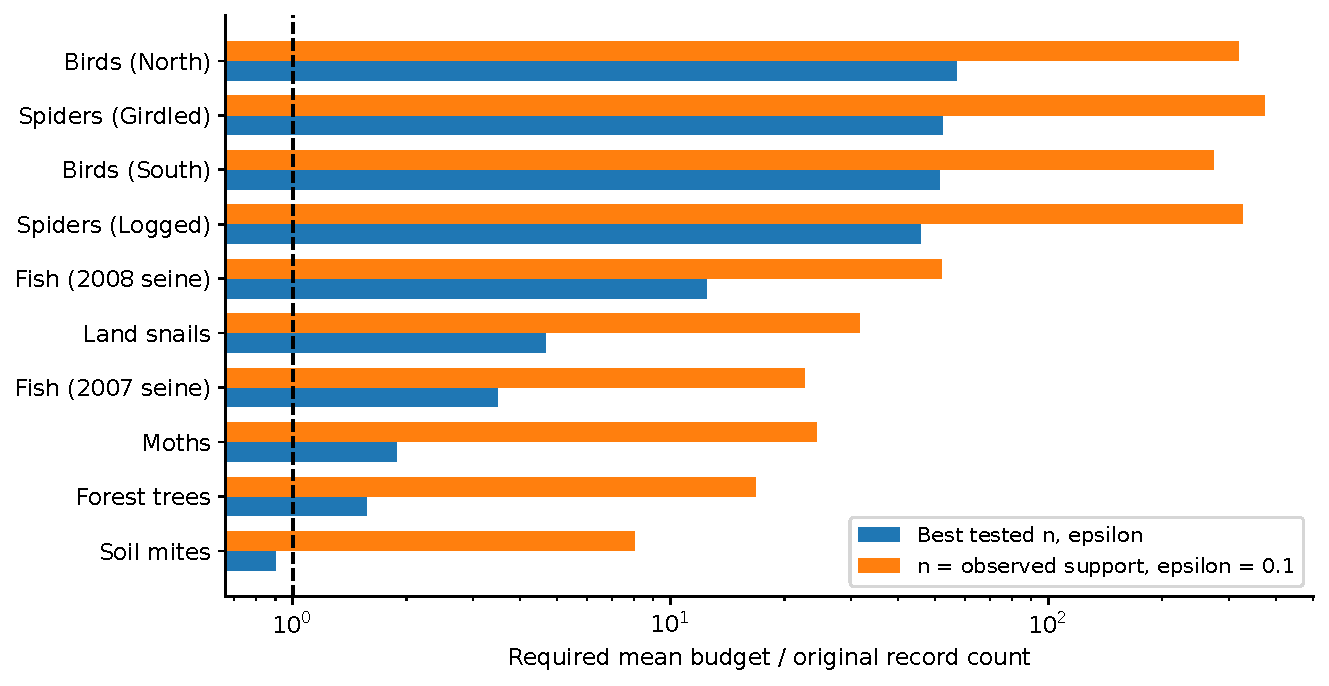
\includegraphics[width=.96\linewidth]{figures/natural_feasibility.pdf}\caption{Budget feasibility: ratios above one mean that the original file has fewer observations than the prescribed mean. Even ratios below one do not establish iid field sampling or guarantee a Poisson draw fits in the file.}\end{figure}

\section{Dependence, held-out groups and stopping rules}

We test two controlled departures from independence while retaining the same marginal species distribution: identical-label duplication and multiple labels drawn within real abundance-weighted groups. Their worst observed false-negative rates are 99.825\% and 42.400\%, respectively. These deliberate stresses are not estimates of natural field dependence. Selecting a group independently for every individual with probability proportional to its abundance recovers the pooled empirical iid target; batching individuals within the same selected group does not.

Five 70/30 group splits per grouped dataset select $n$ using training groups only. Held-out finite populations are independently resampled and scored using their own truth. No errors are observed on promised held-out cells; 5 cells are Gap instances and are not silently assigned a failure label. This measures robustness to finite empirical heterogeneity, not unknown species outside both splits.

A separate actual-label experiment uses $n\in\{10,100,1000\}$, $\epsilon\in\{0.01,0.1\}$ and 300 repetitions. A count comparator stops immediately at the $(n+1)$st distinct label, otherwise reaching its independent Poisson cap. Reporting this stopping rule prevents a batch-checkpoint comparison from overstating the value of the fixed-budget construction.

\begin{figure}[tbp]\centering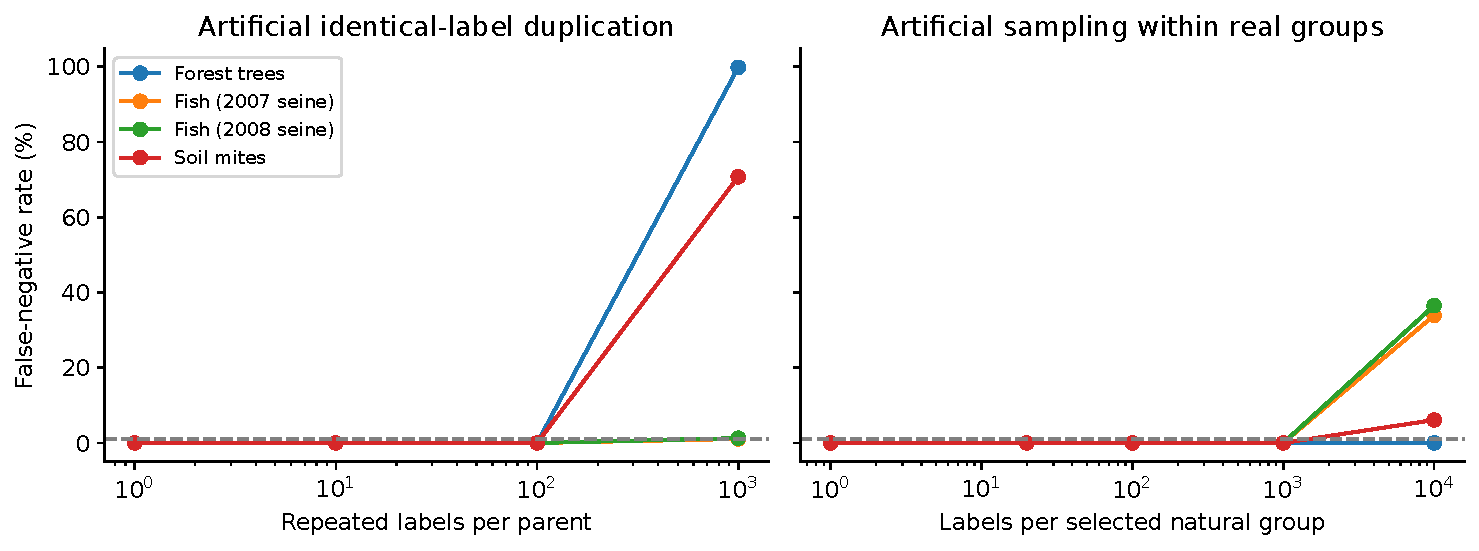
\includegraphics[width=.96\linewidth]{figures/dependence.pdf}\caption{Stress tests preserve the marginal category distribution but violate independence. Group selection is abundance-weighted. Error increases measure artificial perturbations, not an estimate of actual field correlation.}\end{figure}

\begin{figure}[tbp]\centering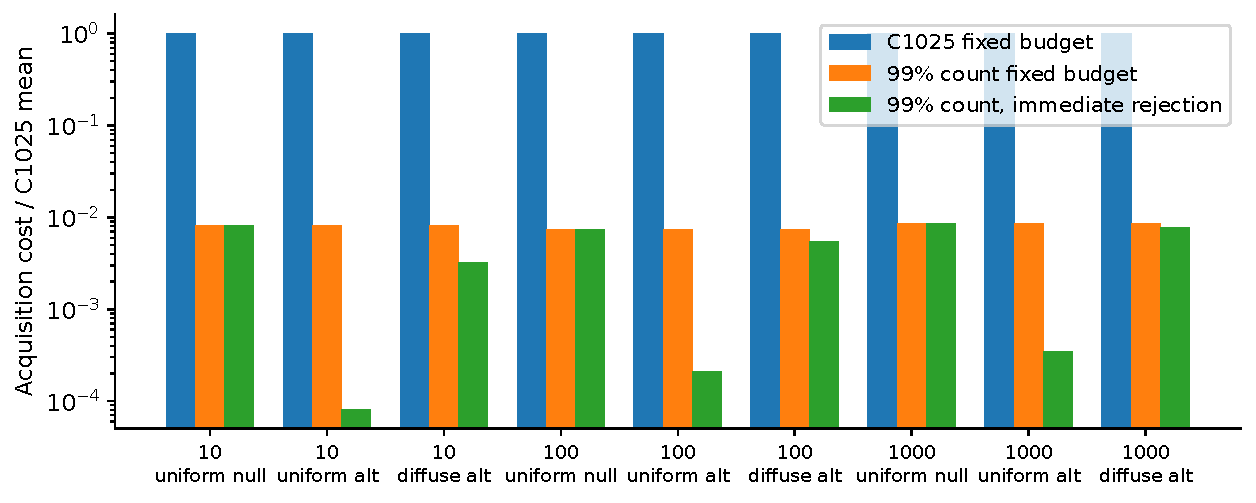
\includegraphics[width=.96\linewidth]{figures/stream.pdf}\caption{Actual label-stream simulation at epsilon=0.01 with 300 trials per cell. The count baseline stops immediately upon observing n+1 species; a prescribed Poisson cap controls acceptance. C1025 bars are prescribed means, not an additional simulated giant stream.}\end{figure}

\section{Full-program and numerical verification}

We executed 1,428 complete public-reference calls on actual independent Poisson category counts, including 300 calls generated from natural empirical probabilities. The resulting decisions and integer lower bounds agree with the count-branch specification. An independent finite occupancy generating-function convolution checks unsaturated small cases. All 43,801 independent algebraic assertions pass, including exact coefficients, branch boundaries, large-degree weights, final decisions, and intentional error controls. Large-parameter fixtures exercise the complete prescribed polynomial degrees and all scales with adaptive interval precision; these are deterministic formula checks, not simulations of $10^{444}$ physical observations.

An additional noninteger-output fixture requires precision escalation from 1608 to 3216 bits; its 443-digit rounded lower bound matches a separately evaluated 4096-bit polynomial formula. This checks rounding after the polynomial, rather than only an easy clipped endpoint. The independent interval formulas share the FLINT arithmetic stack, so this is not an independent proof-assistant certificate.

Runtime measurements isolate count generation from certified public-reference decisions. Every $(n,C_0)$ case runs in a separate process with one warm-up and ten timed repetitions; process peak RSS is retained. Compressed simulation time is reported as computation only. It must not be interpreted as the cost of obtaining the nominal number of observations in nature.

\begin{figure}[tbp]\centering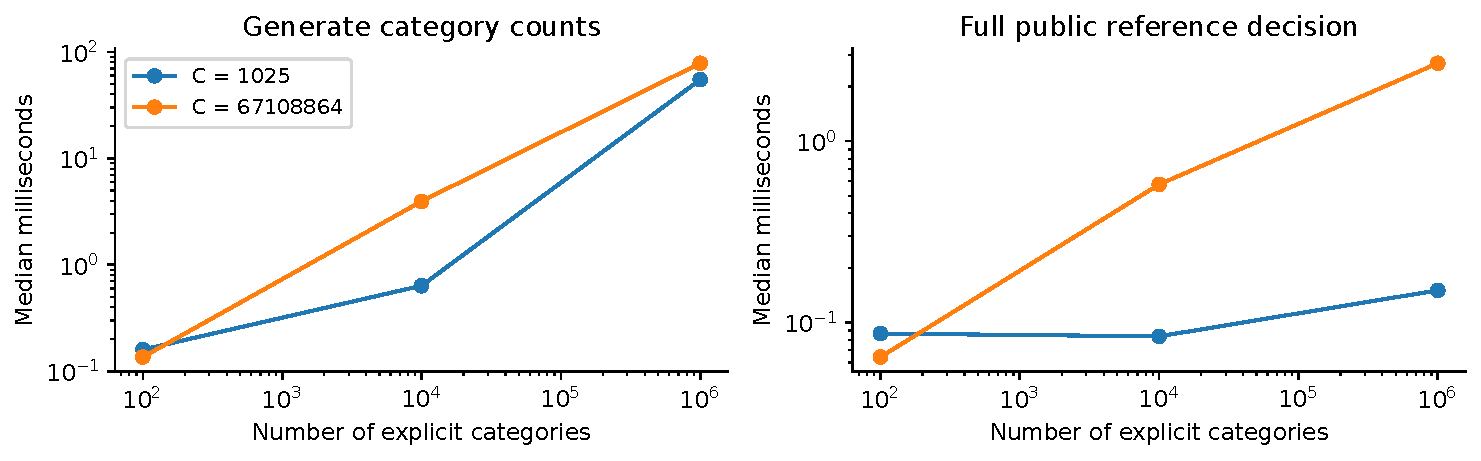
\includegraphics[width=.96\linewidth]{figures/runtime.pdf}\caption{Ten timed repetitions after one warm-up in each isolated process. Independent Poisson category-count generation and certified decision computation are separated. These timings exclude physical data acquisition.}\end{figure}

\section{Reproducibility and limitations}

The artifact contains prospective design files, all primary trial occupancies, per-seed results, exact target audits, source snapshots, environment versions, source-data provenance, figures, code and LaTeX. Run \texttt{python -m c1025.run --phase all}, then \texttt{python -m c1025.supplement}, \texttt{python -m c1025.numeric\_extra}, and \texttt{python -m c1025.report}. Existing completed stages are preserved. The new raw-output audit recomputes every primary decision, confidence bound and lower-bound failure from saved trials. A local frozen protocol is not an external preregistration.

The tested biological collections are diverse but small, historical, and nonrandomly selected; their reference supports omit undiscovered species. No new field survey or external full-population inventory was obtained. The practical grid cannot distinguish 1024 from 1025 at the astronomical worst-case boundary. The proof is not certified by a proof-assistant kernel or independent peer review. The evidence supports a precise constant-refinement evaluation with explicit negative results; publication novelty and fit to a specific conference remain separate questions. No conference template or acceptance claim is implied.
